\section{Contribution}
\label{sec:contribution}

In the following, we will describe the details of how the business model of CCaaS exactly works.
We will first describe the novelty of the solution, before taking a closer look at the functionality,
the pricing and the system architecture of the offering.

\subsection{Novelty}

The idea of offering career counseling as online services is not novel. Neither is the idea of
using AI models to assess a person's skills and interests, or to recommend suitable jobs and training
opportunities based on a user's profile. In fact, 44\% of jobs advertised on LinkedIn are already
filled using skills data as part of the recruitment process \citep{kaserAIpoweredCareerCounseling2023}.
This can typically be achieved by creating word embeddings of the job descriptions and the candidate's
profile (i.e., converting both to vector space), and using a similarity measure between the
vectors. Such vector similarity searches can even be implemented with off-the-shelf vector database
software, such as Weaviate \citep{dilockerWeaviate2023}. However, the idea of offering a platform that
provides career counseling as a service (CCaaS) is novel in several regards:

\begin{itemize}
    \item the business model encourages co-creation of value based on data from LinkedIn and
        personalized services from career counselors
    \item the API layer enables integration with existing career counseling services
    \item the API layer enables counselors to build their own applications on top of the platform
    \item the API layer encourages a mix-and-match approach for career counseling companies, where
        they can choose to use the AI models provided by CCaaS, use their own AI models for certain 
        use cases, or combine the CCaaS API services with services from other APIs (e.g., integrating 
        the training recommendation service with a training provider's API such as Coursera)
    \item CCaaS leverages on the data of LinkedIn to create the best AI models for career
        counseling
    \item the (heavy) investment in training AI models is shared across all users of the platform
        via the API fees
    \item the API approach could fuel further innovation by enabling third-party developers to
        build their own applications on top of the platform, including building applications for 
        niche markets
\end{itemize}

\subsection{Features}

Figure \ref{fig:blueprint_entrant} shows the service blueprint for the customer journey of a job
market entrant using career counseling via CCaaS. A service blueprint is a tool for service design
that describes the customer journey from the customer's perspective and how it connects to the 
frontstage, backstage, and internal support services. The customer journey starts with the job market
entrant matching with a counselor via the LinkedIn matchmaking web application. By choosing a counselor,
the user automatically grants access to its user profile data via the CCaaS API. The counselor can
then access the user's profile data via the API and start the actual counseling process. The counseling
process consists of an assessment of skills and values, retrieving job recommendations, and helping
the client choose the job ads to apply for. The writing assistance service---which is embedded in the 
existing job application forms on LinkedIn---helps the client to write a CV and application letter.
Finally, clients and counselors can leave feedback on the recommendations and the counseling process
via the LinkedIn matchmaking web application.

\begin{figure}
    \centering
    \caption{Service blueprint for the job market entry customer journey. Blue: LinkedIn, orange: counselors (own illustration).}
    \label{fig:blueprint_entrant}
    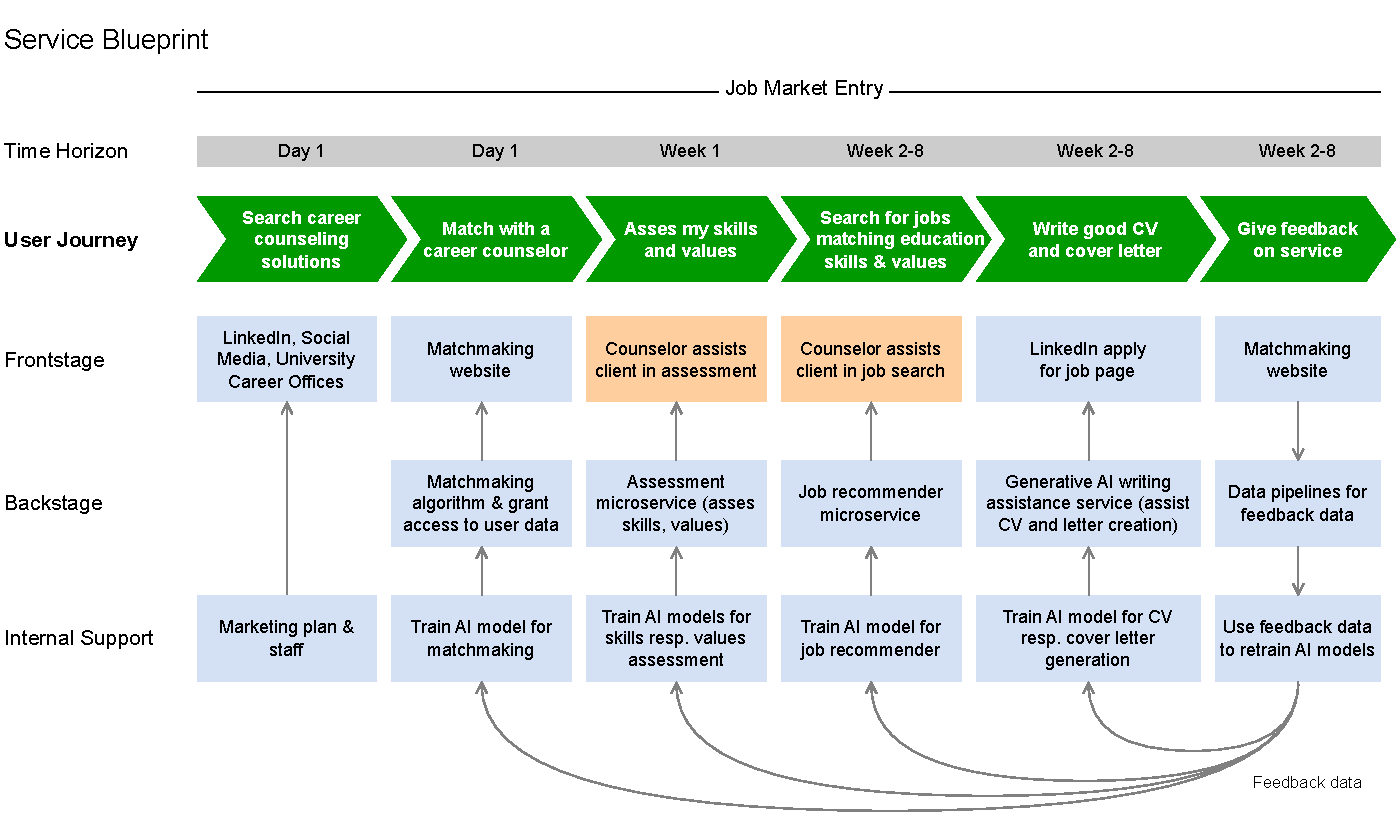
\includegraphics[width=\textwidth]{blueprint_entrant.pdf}
\end{figure}



\subsection{Pricing}

The pricing model for CCaaS is based on a pay-per-use model, where the API usage is metered and
charged to the counseling companies on a monthly basis. Each call on the API layer is logged via
the message broker and a logging microservice. A separate microservice is connected with the billing
and charging system of LinkedIn, and issues a monthly bills to the counseling companies based on
the effective API usage in that month. API requests can have different prices per request, depending
on which API endpoint is used (i.e., what microservice is called). The pricing model is based on
the value that the API endpoint provides to the counseling companies and the complexity of the 
AI models that are underlying the service. 


\subsection{System Architecture}

CCaaS is built as a series of microservices that each handle different types of recommendation
tasks using narrow AI models specifically designed and trained for that task. The services are 
built along the lines of the core value proposition of CCaaS identified in Sections \ref{sec:enablers}
\& \ref{sec:business_model}, namely providing career assessments, career path recommendations, training
recommendations, job recommendations, and writing assistance for CVs and application letters. The
microservices' architecture enables containers to be deployed and scaled independently. They are
connected via a message broker that handles the communication between the services and persistent
storage engines (e.g., to store newly created recommendations and log API requests). Two additional
microservices are responsible for the metering of the API usage and the billing and charging of the
API usage fees to the counseling companies. A web application serves as the gatekeeper between
counselors and clients: clients can choose which counselors they want to work with (matchmaking)
as well as grant access to their LinkedIn profile data to the chosen counselor, so that counselors 
can then subsequently access the client's data via the API and retrieve user-specific recommendations.

A separate system entails the data extraction, transformation and loading (ETL) pipelines that load 
and transforms user data and job data, and ingest them into a distributed large data storage layer
(data lake). The data lake is used to provide large volumes of data in the right format that is 
required to train the AI models. Training of the AI models happens on a cluster of GPU servers. As
introduced in the Section \ref{sec:business_model}, the GPU server farm is provided by the parent
company Microsoft via Azure cloud computing services. The trained models are then deployed to the
microservices that are responsible for the actual recommendation tasks. The overall system architecture
is shown in Figure~\ref{fig:system_architecture} using the C4 modelling language for software architecture
\citep{brownC4ModelVisualising2010}.





\begin{landscape}
    \begin{figure}
        \centering
        \caption{CCaaS system architecture in C4 Level 2 notation (own illustration).}
        \label{fig:system_architecture}
        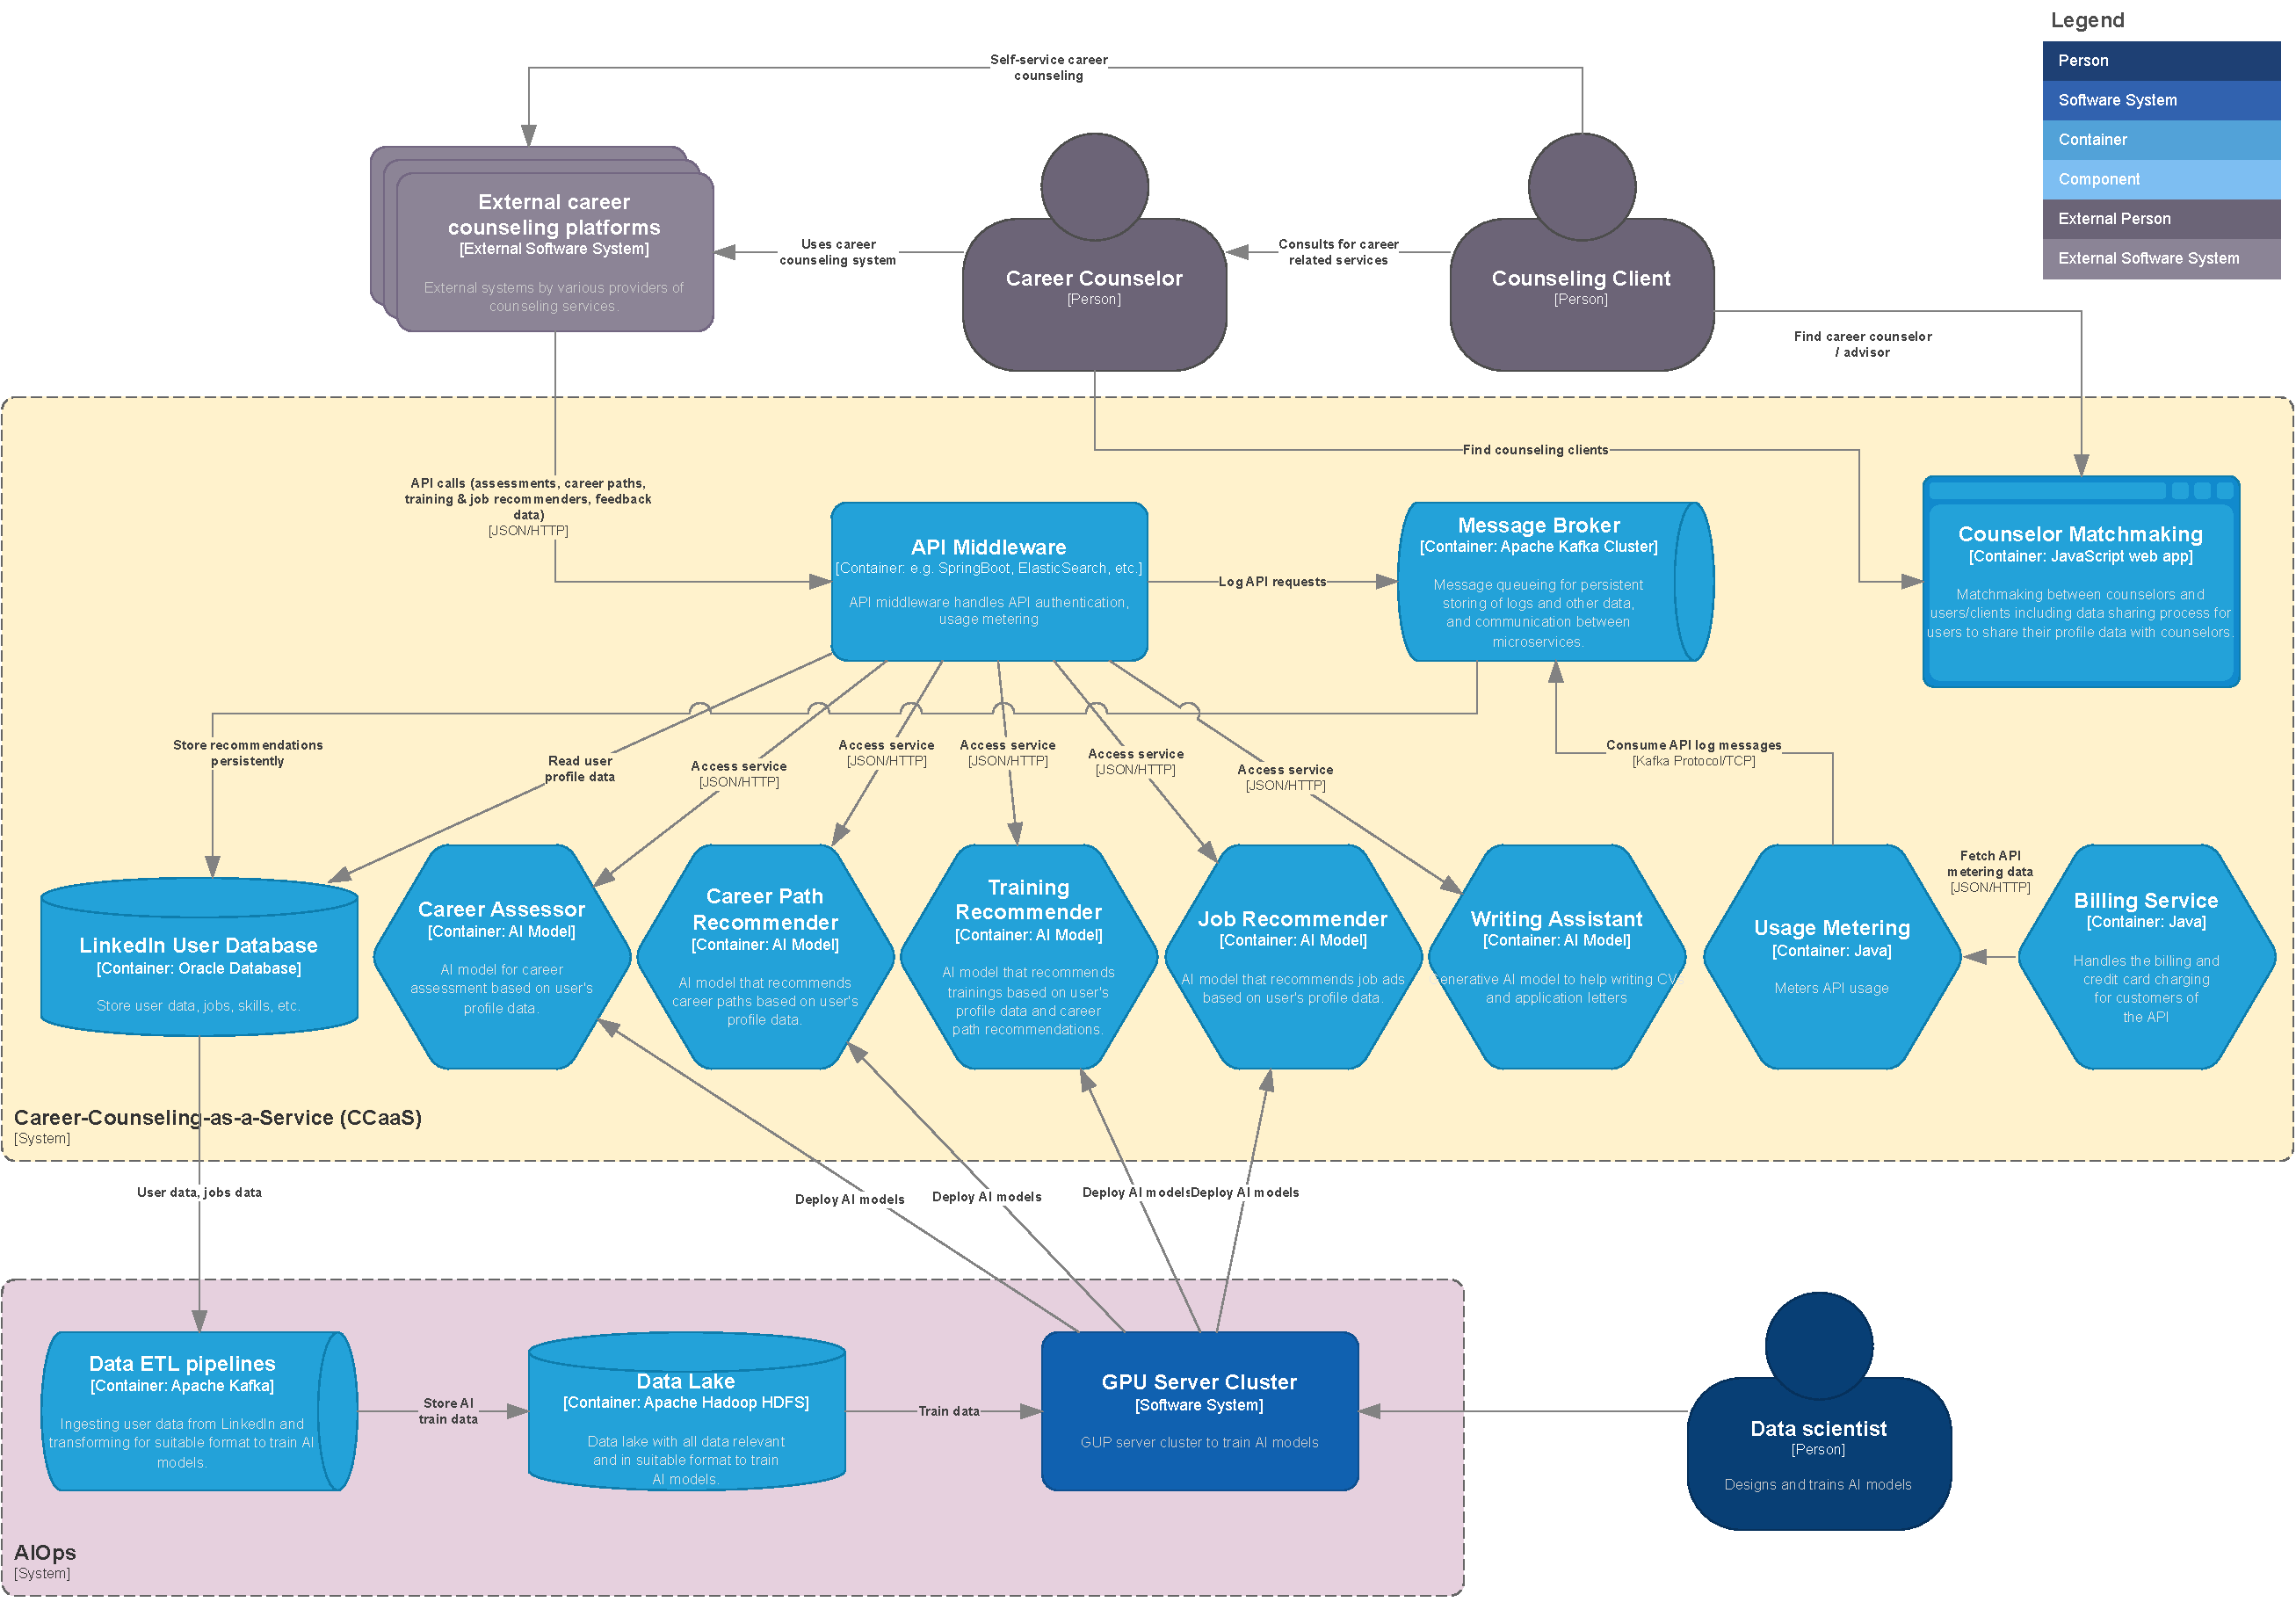
\includegraphics[width=\textwidth]{figures/c4_system_architecture.pdf}
    \end{figure}        
\end{landscape}


